% !TeX root = ../thuthesis-example.tex

\chapter{引言}

\section{研究背景}

根据世界卫生组织(WHO)2018年发布的《2018年全球道路安全现状报告》,全球每年交通事故死亡人数达到了135万。交通事故已经成为5至29岁人群的主要死亡原因。对于发展中国家,
道路交通安全形势更加严峻。\cite{WHO} 根据国家统计局发布的数据,2022年我国共发生交通事故2.4万余起,交通事故死亡人数总计6.1万余人,交通事故造成直接财产损失13余
亿元。\cite{stats_gov}

随着科学技术的发展,自动驾驶技术日渐成熟,各大国内外公司和研究机构都表现出了对自动驾驶技术的浓厚兴趣。自动驾驶技术有望减轻驾驶员的驾驶负担、为残障人士和老人提供自动
驾驶服务、提高道路交通安全、改善道路拥挤堵塞情况,并很可能在不远的未来成为影响交通状况、交通安全的重要元素。但自动驾驶汽车的加入,也会引入新的问题,一方面,
随着自动驾驶技术的逐渐普及,可以预见将长期存在自动驾驶车辆和人工驾驶车辆共存的局面,这会使得交通路况更加复杂,引入更多的不确定性因素和安全隐患;
另一方面,目前自动驾驶技术和测试手段仍然不够成熟,自动驾驶相关法律仍在完善之中,法律责任的确定比较模糊,这些问题使得人们仍然对自动驾驶心存顾虑。

近年来,美国电动汽车及能源公司特斯拉因为自动驾驶技术已发生多起安全事故。2018年5月8日,在美国佛罗里达州劳德代尔堡,一辆2014年产的特斯拉汽车撞上混泥土墙并起火,造成
2名高中生死亡,另有一名高中人受伤;2021年5月7日,在中国广东省韶关市,一辆特斯拉汽车追尾一辆小型货车,造成前者驾驶人当场死亡。这些事故使得人们越来越关注自动驾驶的安全问题。

车队的控制有一个特殊的困难,称为“队列不稳定性”\cite{FENG201981},即系统中的扰动沿着车队不断放大。自动驾驶技术的引入,使得人类可以更加精准地控制车辆,通过控制手段,可以使车队达到“稳定”。
围绕车队稳定性,已经有非常丰富的研究。

碰撞风险评价指标的获得往往是滞后于潜在危险发生的,这不利于交通危险的预测与防范。直观感受上,车队中车辆在速度和位置上的波动是造成车辆碰撞的主要原因,前者可以用车队的队列稳定性来描述,后者可以用碰撞风险来描述,如果能将二者建立联系,就能够用车队的队列稳定性
预测碰撞风险,同时可以通过控制车队的队列稳定程度实现减小碰撞概率的目的,提高道路交通安全程度。

本研究旨在建立自动驾驶车辆和人工驾驶车辆混合车队情景下队列稳定性与碰撞风险的关系,探究碰撞风险在车队中的演化机理,为车队的安全性分析提供理论基础。




\section{国内外研究现状综述}

\subsection{跟驰行为建模研究现状}

驾驶员的驾驶行为和所产生的车辆运行特征是研究交通流的基础。而非自由驾驶情况下,车辆直接的相互作用和导致的交通流变化则是研究的重点。

车辆运动行为主要可以分为车辆跟驰行为和换道行为两大类,跟驰模型的研究对象是前者。用数学模式对跟驰行为加以分析阐明,使得研究人员可以定量地描述跟驰行为,对现代交通的模拟有着重要的意义。

跟驰模型研究主要是运用动力学、统计学等方法,利用驾驶行为问卷调查、模拟驾驶或自然驾驶实验的方式,对前车速度、加速度等行车特征变化引起后车的反应进行研究。

研究者提出了多种跟驰模型,下面分别进行简要介绍。 \\

\noindent \textbf{(1)刺激-反应跟驰模型}

刺激-反应跟驰模型最早由Reuschel\cite{reuschel1950vehicle}和Pipes\cite{Pipes}分别单独提出,其假定驾驶员试图调节车辆速度与前车速度保持一致。

假定驾驶员存在反应延迟,可以得到如下的车辆行驶动力学方程:

\begin{equation}
  a_n(t+T) = c\increment{v_{n, n-1}}(t)
  \label{eq:chap01-1}
\end{equation}
其中,各参数的含义在表\ref{tab:chap01-1}中给出。

\begin{table}
  \centering
  \caption{刺激-反应跟驰模型符号说明}
  \begin{tabular}{cc}
    \toprule
    符号          &  含义                         \\
    \midrule
    $a_n(t)$   & 第$n$辆车在$t$时刻的加速度         \\
    $v_n(t)$   & 第$n$辆车在$t$时刻的速度         \\
    $c$        & 待定比例系数                    \\
    $T$        & 驾驶员的反应延迟时间 \\
    $\increment{v_{n, n-1}}(t)$  &  第$n$辆车与其前车(第$n-1$辆车)在$t$时刻的速度差   \\
    \bottomrule
  \end{tabular}
  \label{tab:chap01-1}
\end{table}

该模型建立了两个被后续研究公认的基础假设:一是驾驶员将考虑本车和前车的速度差来调节车速;二是驾驶员存在反应延迟。但该模型较为简单,不能较好地
符合实际测得的驾驶员加速度特征。Denos C. Gazis等人将自车速度及其前后车距引入刺激-反应跟驰模型,得到了著名的GHR模型\cite{Gazis1961NonlinearFM}:

\begin{equation}
  a_n(t+T) = cv_n^m(t)\frac{\increment{v_{n, n-1}}(t)}{\increment{x_{n, n-1}^l}(t)}
  \label{eq:chap01-2}
\end{equation}
其中,各符号含义在表\ref{tab:chap01-2}中给出。

\begin{table}
  \centering
  \caption{GHR跟驰模型符号说明}
  \begin{tabular}{cc}
    \toprule
    符号          &  含义                         \\
    \midrule
    $a_n(t)$   & 第$n$辆车在$t$时刻的加速度         \\
    $v_n(t)$   & 第$n$辆车在$t$时刻的速度         \\
    $c$        & 待定比例系数                    \\
    $T$        & 驾驶员的反应延迟时间  \\
    $m, l$        & 幂次系数         \\
    $\increment{v_{n, n-1}}(t)$  &  第$n$辆车与其前车(第$n-1$辆车)在$t$时刻的速度差   \\
    $\increment{x_{n, n-1}}(t)$  &  第$n$辆车与其前车(第$n-1$辆车)在$t$时刻的距离   \\
    \bottomrule
  \end{tabular}
  \label{tab:chap01-2}
\end{table}

GHR模型引入了更多参数,表\ref{tab:chap01-3}列出了一些学者的模型拟合结果:

\begin{longtable}{ccc}
  \caption{部分文献中的GHR模型$m$和$l$的取值} \\
  \toprule
  模型出处 & $m$ & $l$ \\
  \midrule
\endfirsthead
  \caption[]{部分文献中的GHR模型$m$和$l$的取值(续)} \\
  \toprule
  模型出处 & $m$ & $l$ \\
  \midrule
\endhead
  \bottomrule
\endfoot
Chandler et al. (1958)      \cite{1958Traffic}         &   0      &   0      \\
\hline
Herman and Potts (1959)      \cite{herman1959single}   &   0      &   1      \\
\hline
Helly (1959)                 \cite{helly1959simulation}&   1      &   1      \\
\hline
Gazis et al. (1961)          \cite{gazis1961nonlinear} & $0-2$    & $1-2$    \\
\hline
May and Keller (1967)        \cite{may1967non}         & 0.8      &  2.8     \\
\hline
Heyes and Ashworth (1972)    \cite{heyes1972further}   & -0.8     &  1.2     \\
\hline
\multirow{3}*{Hoefs (1972)   \cite{hoefs1972entwicklung}} & 减速:1.5 & 减速:0.9 \\
                                                       & 刹车:0.2 & 刹车:0.9 \\
                                                       & 加速:0.6 & 加速:3.2 \\
Ceder and May (1976)         \cite{ceder1976further}   &   0.6    &   2.4    \\
\hline
\multirow{3}*{Aron (1988)    \cite{aron1988car}}       & 减速:2.5 & 减速:0.7 \\
                                                       & 平稳:2.7 & 平稳:0.3 \\
                                                       & 加速:2.5 & 加速:0.1 \\
\hline
\multirow{2}*{Ozaki (1993)   \cite{ozaki1993reaction}} & 减速:0.9 & 减速:1 \\
                                                       & 加速:-0.2& 加速:0.2            
  \label{tab:chap01-3}
\end{longtable}

因为不同的研究者来自不同的地区,不同地区的驾驶员有着不同的驾驶习惯;且随着时代和环境的变化,驾驶员的驾驶行为也发生着变化,所以不同的研究者提出了
显著不同的模型参数拟合结果。不仅如此,早期的车辆间距测算方法较为落后,结果不一定准确,比如,在相邻两辆车之间连接钢卷线的方式,远不如现在采取的激光测距方式方便准确。

刺激-反应跟驰模型形式简单,物理意义明确,具有重要的历史意义,但对真实交通流的模拟能力较弱,存在问题较多,因此研究者提出了许多更加复杂的改进。 \\

\noindent \textbf{(2)安全距离跟驰模型}

安全距离跟驰模型最早由Kometani和Sasaki\cite{ckome1958on}提出,其基本假设是驾驶员在不能完全预判前车运动的情况下,应保持合理的安全间距(指前车车位到后车车头的距离,
一般也被视为足够的刹车距离)以避免碰撞。

模型的表达式为

\begin{equation}
  \increment{x}(t-T) = \alpha v_{n-1}^2(t-T) + \beta_lv_n^2(t) + \beta v_n(t) + b_0
  \label{eq:chap01-3}
\end{equation}
其中,各符号含义在表\ref{tab:chap01-4}中给出。

\begin{table}
  \centering
  \caption{安全距离跟驰模型符号说明}
  \begin{tabular}{cc}
    \toprule
    符号          &  含义                         \\
    \midrule
    $\increment{x}$   & 第$n$辆车在$t$时刻与前车的距离        \\
    $v_n(t)$          & 第$n$辆车在$t$时刻的速度         \\
    $T$        & 驾驶员的反应延迟时间  \\
    $\alpha ,\beta_l , \beta , b_0$        & 待定的系数         \\
    \bottomrule
  \end{tabular}
  \label{tab:chap01-4}
\end{table}

而在实际中, 很多情况下驾驶员并没有做到保持安全距离。且实验表明,在不同车速下,该模型的参数变化幅度较大,导致对实验数据的拟合度不高,并不能很好地定量描
述跟驰行为,所以该模型的实用性并不高。\\

\noindent \textbf{(3)驾驶心理跟驰模型}

由于影响驾驶行为的因素众多。20世纪60年代开始,研究人员开始更多地关注驾驶员的心理因素。研究多基于驾驶员按照前后车的相对运动(如速度和距离的变化)
来调节自身跟随速度,当这些刺激因素的指标超过事先给定的阈值之后, 驾驶员才会有所感知,并作出反应的基本假设。\cite{Todosiev1963the}

不同状态的跟驰车辆(比如不断接近或远离前车)拟合出的阈值也表现出较大的区别。因此在20世纪70年代,研究人员开始关注如何来定义平均阈值。对驾驶心理模型的
研究开始集中在对驾驶员试验数据的心理和生理统计分析上。

目前常见的驾驶心理跟驰模型常常要划分特定的驾驶状态和相应的阈值,比如驾驶状态空间可以被划分为:\\

\begin{description}
\item [A. 自由驾驶状态(free driving mode):]
  本车和前车距离大于最大相互作用距离,此时驾驶员将尽力达到可能的最大行车速度; \\
\item [B. 接近状态(approaching mode):]
  本车和最近的前车距离小于最大相互作用距离、大于刹车距离,并且本车速度远大于前车速度。一般而言,驾驶员将一方面尽快缩小和前车的距离,
  一方面逐步减速使得本车和前车的速度保持一致。 \\
\item [C. 离开状态(leaving mode):]
  本车和最近的前车距离小于最大相互作用距离且大于刹车距离,并且本车速度远小于前车速度。此状态描述驾驶员从跟随驾驶状态转入自动驾驶状态的过程。
\end{description}  

早期驾驶心理跟驰模型采用固定的阈值,其缺点在于每个阈值都可能随交通环境的变化而变化,难以调查确定。 目前的驾驶心理跟驰模型尚无法对所有这些
特性进行分析建模,常见的模型主要集中在感知周围信息、制动过程中驾驶人行为以及驾驶人对于安全车头间距、车头时距或者预碰撞时间的选择等几个关键问题上。\\

\noindent \textbf{(4)人工智能跟驰模型}

20世纪90年代开始,人工智能领域的各个算法开始在驾驶员行为建模研究中得以应用,其原理是:在人类驾驶员跟驰过程中,驾驶行为可以视为一个复杂的非线性系统,
由于影响驾驶行为的因素有很多,其之间的关系非常复杂,传统方法很难对如此复杂的非线性系统进行拟合。但随着计算能力的提升和深度学习方法的发展(比如VGG网络
证实了神经网络的深度能够在一定程度上提升网络性能,残差结构能够有效解决梯度回传中梯度消失的问题,使得更深的网络称为可能),拥有更加强大拟合能力的人工神
经网络被尝试用于更加准确地模拟驾驶行为上。\cite{Kikuchi1992fuzzy}

但采用人工神经网络的跟驰行为建模方法也存在不可忽视的问题,端到端人工神经网络存在不具有解释性的问题,这使得人工智能跟驰模型对驾驶人的行为分析方面较弱,
且易在建立过程中参杂主观因素(如按照主观感受设计模型结构)。由于人工智能跟驰模型不能写出显示的表达式,也不利于基于跟驰模型的相关分析工作,如跟驰行为
的稳定性分析。 \\ 

\noindent \textbf{(5)速度优化跟驰模型}

速度优化跟驰模型(Optimal Velocity Model, OVM)是Bando等人在1995提出的,是描述跟驰行为的经典模型之一。\cite{PhysRevE.51.1035}

其模型的控制方程为

\begin{align}
  \dot{v}_n(t) &= \kappa \left\{ \mathrm{V} \left[ h_n(t) \right] - v_n(t) \right\} \notag \\
  \mathrm{V} \left[ h_n(t) \right] &= v_0 \left\{ 1 - \exp \left[ - \frac{\alpha}{v_0}\left(h_n(t)-s_0\right) \right] \right\}
  \label{eq:chap01-4}
\end{align}
其中,各符号含义在表\ref{tab:chap01-5}中给出。

\begin{table}
  \centering
  \caption{速度优化跟驰模型符号说明}
  \begin{tabular}{cc}
    \toprule
    符号          &  含义                         \\
    \midrule
    $\dot{v_n}(t)$    & 第$n$辆车在$t$时刻的加速度        \\
    $v_n(t)$          & 第$n$辆车在$t$时刻的速度         \\
    $h_n(t)$          & 第$n$辆车在$t$时刻与前车的车头间距  \\
    $\mathrm{V}(\cdot)$        & 速度优化函数         \\
    $\kappa, \alpha$  & 敏感系数             \\
    $v_0$             & 自由流速度           \\
    $s_0$             & 最小安全距离        \\
    \bottomrule
  \end{tabular}
  \label{tab:chap01-5}
\end{table}

可以看出,对于某一位驾驶人,在给定车头间距后,存在一个优化速度函数,该函数来描述该驾驶人希望保持的理想速度大小,且该函数在定义域内是单调递增的。
这与实际情况较为相符:车头间距越小,驾驶人倾向于以更小的速度来跟驰以减小追尾风险;车头时距越大,驾驶人倾向于以更大的速度来跟驰以减小两车之间的距离。
这里的“倾向”都是通过速度优化函数来刻画的。

OVM表达形式直观,将驾驶人的心理因素与行为因素有效结合;且参数量比较适中,定量描述能力较强。同时,OVM的形式方便交通流的稳定性分析,被驾驶行为相关
研究学者广泛应用。

表\ref{tab:chap01-6}对上述的跟驰模型进行了总结。

\begin{table}
  \centering
  \caption{跟驰模型总结}
  \begin{tabular}{cll}
    \toprule
    跟驰模型           &  \multicolumn{1}{c}{基本假设}           & \multicolumn{1}{c}{特点}               \\
    \midrule
    \multirow{2}*{刺激-反应跟驰模型}     &  1. 驾驶员依据与前车的速度差来调节车速   &  形式简单、物理意义明确,但  \\
                                      &  2. 驾驶员存在反应延迟                &  对真实交通流的模拟能力较弱   \\
    \multirow{2}*{安全距离跟驰模型}      &  驾驶员在不能完全预判前车运动的情况下    &  不同环境下,模型参数变化幅 \\
                                      &  保持合理安全间距                     &  度大,对实验数据拟合度不高 \\
    \multirow{2}*{驾驶心理跟驰模型}      &  当刺激因素指标超过给定阈值后,驾驶员    &  阈值在不同环境下不同,难以 \\
                                      &  才会感知到并作出反应                 &  确定调查                  \\
    \multirow{2}*{人工智能跟驰模型}      &  跟驰行为被视为一个复杂的非线性系统,   &  神经网络解释性差,且不能写  \\
                                      &  用人工神经网络进行拟合                &  出显式表达式,不利于分析     \\
    \multirow{2}*{速度优化跟驰模型}      &  存在一个速度优化函数,可以描述驾驶人    &  表达形式直观,将驾驶人心理 \\
                                      &  希望保持的理想速度大小               &  与行为结合,且参数量适中      \\                                   
    \bottomrule
  \end{tabular}
  \label{tab:chap01-6}
\end{table}

\subsection{车队稳定性分析研究现状}
\label{sec:1.2.2}

在交通流中,关于稳定性的研究大致有两种,一种是在时间维度上,单车在受到前车运动引起的小扰动影响下的运动稳定性;另一种是在空间上,车队在一个
小扰动下的运动稳定性,这里的小扰动通常是源于头车的。本研究关心的是头车的扰动对于整个混合车队以及整个混合车队的稳定性的影响,所以这里更关心第二
种稳定性,这种稳定性也被称为队列稳定(String Stability, SS)。

在车队中,如果把每一辆跟驰车辆看作是一个传递单元,则头车受到的无论是速度上的,还是位置上的扰动都会随着车队传递。如果车队是稳定的,扰动会
在每一个传递单元衰减,更具体来说,如果车队在速度上是稳定的,那么速度的振荡幅度会随着空间上的传播而减小;同理,如果车队在位置上是稳定的,
那么位置的振动幅度会随着空间上的传播而减小。

在跟驰模型的基础上,可以定量地对车队的稳定性进行分析。队列稳定分析与交通流建模特别相关,因为实际交通中的走走停停和振荡是交通流队列稳定性的
一种具体表现。从跟驰模型发展的角度来看,一个真实的跟驰模型应该能够描述队列稳定性。因此,自跟驰模型提出以来,就有很多基于此的队列稳定性分析工
作。Sun Jie等人对车队稳定性的研究现状进行了全面的描述\cite{SUN2018212},下面进行简要介绍: \\

\noindent \textbf{(1)基于传递函数的方法}

基于传递函数的方法都基本思想是观察系统的输入与输出之间的频率响应。如果将车队中的每一辆跟驰车辆都近似看作一个线性系统,那么可以写出其传递函数
\begin{equation}
  G(s) = \frac{b(s)}{a(s)}
  \label{eq:chap01-5}
\end{equation}
令$s=i\omega$,可以得到该单元的输出$x(t)$为
\begin{equation}
  x(t) = G(i\omega)e^{iwt} = M\cos(\omega t+\varphi) + iM\sin(\omega t+\varphi)
  \label{eq:chap01-6}
\end{equation}
其中,$M = |G(i\omega)|$,$\varphi = \arctan \frac{\Im G(i\omega)}{\Re G(i\omega)}$,分别为传递函数的幅值增益和相移。如果
$M = |G(i\omega)| < 1$,就有$\Vert x(t) \Vert < \Vert h(t) \Vert$,$h(t)$是系统的输入。对于车队系统,若头车收到的扰动为
\begin{equation}
  u_0(t) = e^{i\omega t}
  \label{eq:chap01-7}
\end{equation}
那么传递到第$n-1$辆车,其波动就是
\begin{equation}
  u_n(t) = G^n(s)e^{i\omega t}
  \label{eq:chap01-8}
\end{equation}
所以扰动在车队中逐渐衰减的一个充分条件是
\begin{equation}
  |G(i\omega)| < 1
  \label{eq:chap01-9}
\end{equation} \\

\noindent \textbf{(2)基于拉普拉斯变换的方法}

将车队中每辆跟驰车辆看做一个线性单元,其传递函数为$G(s)$,$g(t)$是传递函数的拉普拉斯逆变换,假设第$n$辆车受到的扰动为$\varepsilon_n(t)$,其拉普拉斯变换为$E_n(s)$,
那么连续的两辆车收到的扰动在频域的关系为
\begin{equation}
  G(s) = \frac{E_n(s)}{E_{n-1}(s)} 
  \label{eq:chap01-10}
\end{equation}
那么有
\begin{equation}
  \begin{aligned}
  \Vert \varepsilon_n(t) \Vert_{\infty} &= \max_{t}|\varepsilon_n(t)| \\
                                        &= \max_{t} \left|\int_0^tg(\tau)\varepsilon_{n-1}(t-\tau)\mathrm{d}\tau \right| \\
                                        &\leqslant \max_{t}\int_0^{\infty}|g(\tau)||\varepsilon_{n-1}(t-\tau)| \mathrm{d}\tau \\
                                        &\leqslant \int_0^{\infty} |g(\tau)|\mathrm{d}\tau \cdot \max_t|\varepsilon_{n-1}(t-\tau)| \\
                                        &= \Vert g \Vert_1 \Vert \varepsilon_{n-1} \Vert_{\infty}
  \end{aligned}
  \label{eq:chap01-11}
\end{equation}
若要队列保持稳定,需要
\begin{equation}
  \Vert g \Vert_1 < 1 
  \label{eq:chap01-12}
\end{equation}
同时,注意到有
\begin{equation}
  \begin{aligned}
  \left| G(i\omega) \right|  &=  \left| \int_0^{\infty}g(t)e^{-i\omega t}\mathrm{d}t \right| \\
                             &\leqslant \int_0^{\infty}|g(t)||e^{-i\omega t}| \mathrm{d}t \\
                             &= \int_0^{\infty} |g(t)| \mathrm{d}t \\
                             &= \Vert g \Vert_1
  \end{aligned}
  \label{eq:chap01-13}
\end{equation}
结合式(\ref{eq:chap01-12})与式(\ref{eq:chap01-13}),可以得到队列稳定的一个充分条件为
\begin{equation}
  |G(i\omega)| < 1 
  \label{eq:chap01-14}
\end{equation}
可以发现这与基于传递函数的方法得到的结论(式(\ref{eq:chap01-9}))是一致的。 \\


\noindent \textbf{(3)基于特征方程的方法}

假设第$n$辆车受到速度上的扰动为
\begin{equation}
  u_n(t) = u_n^0e^{\lambda t} = \hat{u} e^{in\varphi} e^{\lambda t} = e^{\lambda t + in\varphi} \hat{u}
  \label{eq:chap01-15}
\end{equation}
第$n$辆车在位置上的扰动为
\begin{equation}
  y_n = e^{\lambda t + in\varphi}\hat{y}
  \label{eq:chap01-16}
\end{equation}
由此可以得到

\begin{equation}
  \left(\begin{array}{cc}
    \lambda & 1-e^{-i\varphi} \\
    f_s & \lambda - (f_v-f_{\increment{v}}+f_{\increment{v}} e^{-i\varphi}) \\
  \end{array} \right)
  \left(\begin{array}{cc}
    \hat{y} \\
    \hat{u} \\
  \end{array} \right) = 0
  \label{eq:chap01-17}
\end{equation}\\ 

\noindent 式(\ref{eq:chap01-15})、式(\ref{eq:chap01-16})和式(\ref{eq:chap01-17})中出现的符号含义列在了表\ref{tab:chap01-7}中。
\begin{table}
  \centering
  \caption{基于特征方程的方法推导所用符号说明}
  \begin{tabular}{cc}
    \toprule
    符号          &  含义                         \\
    \midrule
    $\sigma$          & 振荡幅度的增长率         \\
    $\omega$          & 频率         \\
    $\lambda=\sigma+i\omega$    & 复合增长率        \\
    $\hat{u}, \hat{y}$          & 复常数         \\
    $v$            & 第$n$辆车的速度         \\
    $\increment{v}$            & 第$n$辆车与前车的速度差         \\
    $f$            & 将若干变量映射到车辆加速度的函数,即车辆的动力学方程         \\
    $f_s = \frac{\partial f}{\partial s} |_e$          & $f$对$s$的偏导数在稳定时的取值         \\
    $f_v = \frac{\partial f}{\partial v} |_e$          & $f$对$v$的偏导数在稳定时的取值         \\
    $f_{\increment{v}} = \frac{\partial f}{\partial \increment{v}} |_e$          & $f$对$\increment{v}$的偏导数在稳定时的取值         \\
    \bottomrule
  \end{tabular}
  \label{tab:chap01-7}
\end{table}

该齐次二元线性方程(式(\ref{eq:chap01-17}))只有在系数方阵的行列式奇异的时候才有非零解,我们记
\begin{equation}
  \begin{cases}
    p(\varphi) = -f_v + f_{\increment{v}} - f_{\increment{v}}e^{i\varphi} \\
    q(\varphi) = f_s(1-e^{\-i\varphi})
  \end{cases}
  \label{eq:chap01-18}
\end{equation}
那么有
\begin{equation}
  \lambda^2 + p(\varphi)\lambda + q(\varphi) = 0
  \label{eq:chap01-19}
\end{equation}
求解得到$\lambda_{\pm}$之后在$\varphi \rightarrow 0$附近将$\lambda_+$展开,为满足稳定性判据,其实部需要为负数,最终得到车队稳定的一个充分条件
\begin{equation}
  f_v^2 - 2f_s -2f_vf_{\increment{v}} >0>\-\omega^2 or \frac{1}{2} - \frac{f_{\increment{v}}}{f_v} - \frac{f_s}{f_v^2} > 0
  \label{eq:chap01-20}
\end{equation}

\subsection{车队碰撞风险评估指标研究现状}

跟驰行为的安全性研究主要是通过理论模型、数值仿真以及部分实测试验等方法对车队的安全性进行评价。从时间、距离、加速度等不同维度,学者提出了多种安全性评价方式,
下面分别进行简要介绍。

一种常用的基于时间的度量指标是碰撞时间(Time to Collision, TTC),指的是在当前车辆在当前速度、与前车距离、行驶轨迹下与前车发生碰撞所需要的时
间\cite{Horst1990ATA}。更准确的说, 一共有三种不同的TTC度量方式:TTC1为两车之间保险杠的距离除以两车的接近速度;TTC2考虑了两车的加速度,即以
当前两车的速度和加速度以及距离下,辆车发生碰撞需要的时间。可以看到二者的主要区别在于TTC2考虑了TTC1没有考虑的两车的加速度信息。第三种TTC的度量方式为
TTC1的倒数,这是因为当本车与前车相对速度很小时, TTC1会趋于无穷大,这会对分析带来诸多不便,因此TTC1也常被用于危险估计。

第二种基于减速的度量是车头时距(Time Headway, TH),计算方法为
\begin{equation}
  \mathrm{TH}_n(t) = \frac{S_{n, n-1}(t)}{v_n(t)}
  \label{eq:chap01-21}
\end{equation}
其中,各符号含义在表\ref{tab:chap01-8}中给出。
\begin{table}
  \centering
  \caption{TH计算公式符号说明}
  \begin{tabular}{cc}
    \toprule
    符号          &  含义                         \\
    \midrule
    $\mathrm{TH}_n(t)$          &    第$n$辆车在$t$时刻的车头时距         \\
    $v_n(t)$           &    第$n$辆车在$t$时刻的速度       \\
    $S_{n, n-1}(t)$    &    第$n$辆车的车头在$t$时刻与前车的距离      \\
    \bottomrule
  \end{tabular}
  \label{tab:chap01-8}
\end{table}

车头时距是一个很重要的概念,因为它确定了后车的驾驶员在前车最大减速度下突然刹车时拥有的反应和减速时间。

潜在危险时间(Potential Dangerous Time, PDT)比例也是描述安全性的一种指标。潜在危险指前后车不满足式(\ref{eq:chap01-22})的条件时,后车具有追尾前车的风险。存在潜
在危险的时间占总时间的比例称为潜在危险时间比例。
\begin{equation}
  \increment{x}_n \geqslant A + B - (C - l_{n-1})
  \label{eq:chap01-22}
\end{equation}
其中,各符号含义在表\ref{tab:chap01-9}中给出。
\begin{table}
  \centering
  \caption{式(\ref{eq:chap01-22})符号说明}
  \begin{tabular}{cc}
    \toprule
    符号          &  含义                         \\
    \midrule
    $\increment{x}_n$          &    第$n$辆车距离前车的距离         \\
    $A$                        &    前车紧急减速后,后车驾驶员在反应时间内行驶的距离      \\
    $B$                        &    前车紧急减速后,后车在紧急减速过程中行驶的距离      \\
    $C$                        &    前车紧急减速过程中行驶的距离      \\
    $l_n$                      &    第$n$辆车的车身长度     \\
    \bottomrule
  \end{tabular}
  \label{tab:chap01-9}
\end{table}

关于安全性指标的选取工作有很多,有学者提出用TTC的倒数与车头时距倒数的加权和来表征危险\cite{Kondoh2008iden};
还有工作\cite{DBLP:journals/corr/abs-1708-06374}提出了一种责任敏感安全(Responsibility Sensitive Safety, RSS)
模型,在RSS中定义了责任安全来防止过于保守的驾驶策略。

由于自动驾驶车辆比人工驾驶车辆反应速度更快,也有工作\cite{Morando2018Studying}指出自动驾驶车辆的TTC阈值应取为1秒,
而人工驾驶车辆常用的TTC阈值为1秒。

\subsection{研究现状总结}

无论是对于纯人工驾驶车队、纯自动驾驶车队还是人工驾驶和自动驾驶混合车队,围绕稳定性与安全性都已经进行了很多的工作。

车辆的跟驰行为建模方面,基于不同的假设有不同的跟驰模型,不同的跟驰模型也有不同的使用范围。跟驰模型的质量将直接决定仿真的精准程度,有着极高的应用价值。

车队稳定性方面,针对队列稳定性研究人员提出了若干定义与分析方法,这为本工作中对混合车队的稳定性分析提供了坚实的理论基础。现有的工作
多认为队列稳定性与交通的拥堵情况有关,认为不稳定的车队更容易产生交通拥堵。就分析方法而言,有基于频域和时域的若干种分析方法,不同的方法有不同的
适用情况,需要根据实际的车队信息流拓扑结构等条件选择合适的定义与分析方法。

车队的安全性评估指标方面,通过理论模拟、数值仿真和实验测试等方法,学者提出了很多种安全评价指标。不同的安全评价指标反映了对于安全评估的不同侧重点。
在使用时应首先明确研究的目标,选择合适的安全评估指标。

综上所述,本课题试图建立车队的队列稳定性与安全性的关系,探究碰撞风险在车队中的演化机理,这是一个相对空白的研究方向,但有非常大的研究价值和实际意义。

\section{课题研究目标与难点}

\subsection{研究目标}

本文的研究的主要对象是人工驾驶与自动驾驶的混合车队,将基于混合车队的稳定性对碰撞风险及其演化机理进行研究。对于混合车队的稳定性,
将通过不同的跟驰模型定量描述人工驾驶车辆与自动驾驶车辆的跟驰行为,并基于此完成稳定性的分析;对于混合车队的碰撞风险演化机理,主要通过仿真的方
式进行研究。

本文的研究将主要分为以下几个部分:\\ 

\noindent \textbf{(1)稳定性条件探究}

纯人工驾驶车辆车队和纯自动驾驶车辆车队由于每一个车辆单元都是相同的,其队首-队尾传递函数(整个车队的传递函数)是由若干相同的传递函数(每辆跟驰车辆的传递函数)
相乘得到的,其形式比较简单。而对于混合车队,由于人工驾驶车辆和自动驾驶车辆的跟驰行为建模不同,车队的队首-队尾传递函数中会包含多于一种形式的传递函数。本文将
推导混合车队队列稳定的条件。 \\

\noindent \textbf{(2)稳定性指标与碰撞风险指标关系探索}

此部分是本工作的核心内容。碰撞风险评价指标的获得往往是滞后于潜在危险发生的,这不利于交通危险的预测与防范。混合车队的稳定性反映了头车速度以及位移的扰动随车
队的传播,这些扰动是造成车队不安全(碰撞风险)的可能原因,因此猜想混合车队的稳定性和碰撞风险之间是有一定联系的。

而无论是对于混合车队的稳定性还是碰撞风险,都有多种影响因素,本文希望通过仿真,全面地对有关因素及对于混合车队稳定性和碰撞风险关系进行分析。\\

\noindent \textbf{(3)混合车队碰撞风险演化机理探究}

对于队列稳定性不同的车队,碰撞风险在其中演化的机理也可能是不同的,即使队列稳定性相通的车队,也可能因为车队的排列方式(比如车队中人工驾驶车辆和自动驾驶车辆的分散
程度和靠近头车程度)不同,呈现出不同的碰撞风险演化机理。本课题探究了不同队列稳定性和车队的排列方式下的碰撞风险演化机理,希望探究结论能对降低混合车队碰撞风险有指导价值。

\subsection{研究难点}

\noindent \textbf{(1)稳定性的分析与指标选取}

通过文献调研,对于车队的队列稳定性,从不同维度上,对于不同的实际情境,有不同的定义。要深入、全面地理解已有的稳定性分析工作是一个难点。其次,稳定性指标的选
择也非常重要,因此首要工作是选择适合本工作中仿真情景的队列稳定性指标。\\

\noindent \textbf{(2)碰撞风险指标的选取}

学者提出了很多种安全评价指标,不同的安全评价指标反映了对于安全评估的不同侧重点。选择合适的碰撞风险指标是本工作的一个难点。 \\

\noindent \textbf{(3)影响稳定性与碰撞风险的相关因素众多,且耦合性强}

影响稳定性指标的因素和影响碰撞风险指标的因素都有很多,且这些因素耦合在一起,使得分析工作复杂繁琐。如何合适地在实验中控制变量、如何全面地从合适的角度展示稳定性、
碰撞风险以及相关因素之间的关系是本工作的一个难点。\\

\noindent \textbf{(4)仿真结果不直观,难以解释}

仿真会得到难以解释或与生活经验相反的结果,如何对已有结论进行解释是本工作的一个难点。对此,本工作中实现了简易的仿真过程可视化,方便直观感受仿真过程。

\section{论文结构及章节安排}

本工作技术路线如图\ref{fig:chap01-1}所示。

\begin{figure}
  \centering
  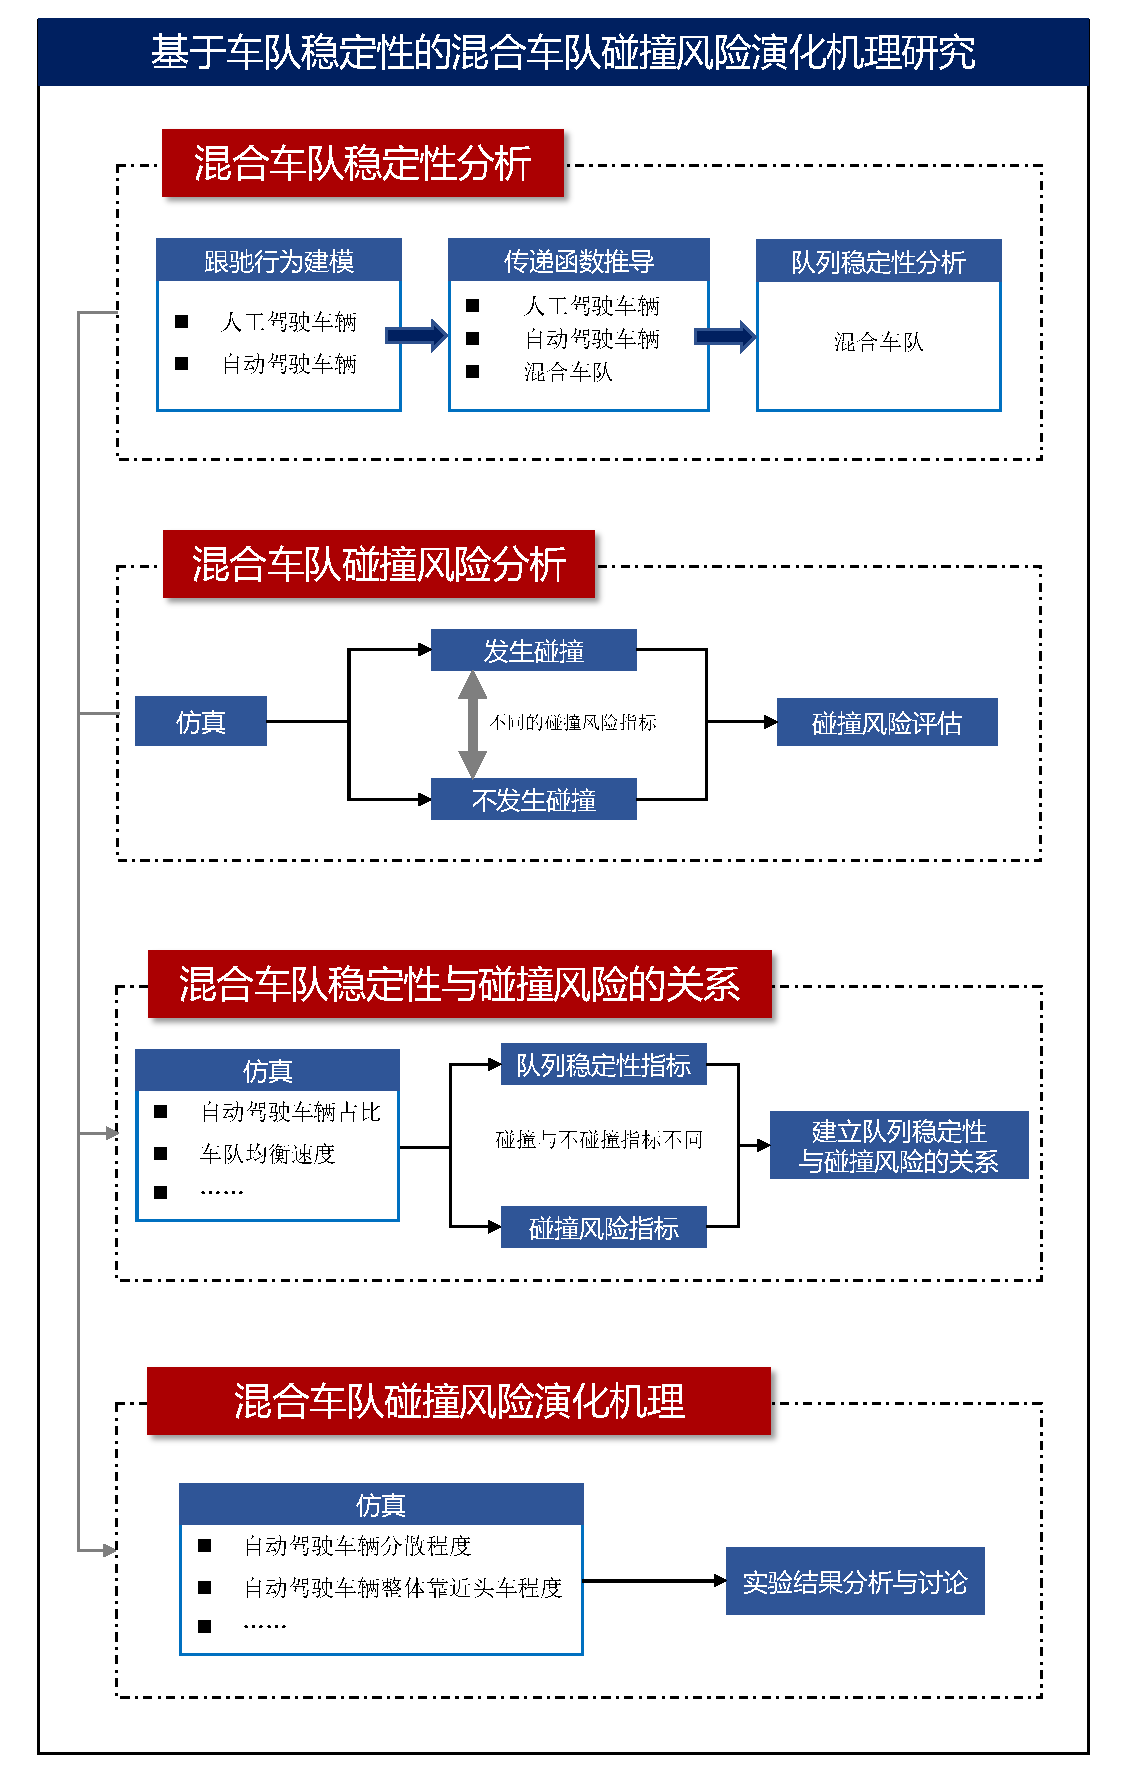
\includegraphics[width=0.778\linewidth]{chap01-1-tec_map.pdf}
  \caption{项目技术路线}
  \label{fig:chap01-1}
\end{figure}

对于混合车队稳定性的分析工作是在选定人工驾驶车辆和自动驾驶车辆的跟驰模型后基于理论推导展开的;关于混合车队稳定性与碰撞风险之间关系的探究以及车队碰撞风险演化机理的研究都是
基于仿真展开的,在后文中也将介绍仿真平台的搭建工作。

本文共6个章节,内容安排如下:

第2章介绍仿真平台。本工作主要是基于仿真展开的,建立车队稳定性与碰撞风险之间的关系,以及探究碰撞风险的演化机理,都以仿真结果为基础,所以仿真平台的质量以及
仿真的真实性都十分重要。在第2章中会对跟驰行为的建模、仿真平台的的搭建、仿真的主要参数以及仿真平台的真实性进行介绍。

第3章基于第2章选择的跟驰模型对车队的队列稳定性进行了分析与仿真。首先分别对人工驾驶车辆和自动驾驶车辆根据二者的跟驰模型推导出传递函数,得到车队整体的传递函数;
再使用引言中介绍到的车队稳定性分析方法得到车队队列稳定的判据;最后通过仿真进行验证。

第4章对仿真结果进行了分析。碰撞(追尾)是仿真过程中一个非常直观的现象,显然,如果车队中已经发生了碰撞,那么潜在风险的统计分析就失去了意义,所以首先根据仿真过程中发生碰撞与否可以将所有样本分为
两大类,即碰撞样本和非碰撞样本。在本章对这两大类分别建立了稳定性与碰撞风险的关系,并对碰撞风险的演化机理进行了探究。

第5章对工作进行了总结,并对本工作可能的改进方向和后续工作进行了展望。


